% TODO
% add images
% also MITM without authentication?

\documentclass[11 pt]{article}
\usepackage{graphicx}
\title{
	Diffie –- Hellman key exchange for multiple parties \\
	\large HW4 - CNS Sapienza}

\author{Luigi Russo 1699981}
\date{23/11/2018}

\begin{document}

\maketitle

\section{Overview}
Diffie -- Hellman (\textbf{DH}) key exchange is a method of exchanging keys over a public channel in a secure way. It allows two parties, say Alice (A) and Bob (B) to agree a common secret key to be used later, after sharing over the public channel some informations. The method is basically this:
\begin{enumerate}
	\item Alice generates a number \textit{a} (secret) and so does Bob with \textit{b}
	\item Alice also chooses a prime number\footnote{Here I describe the canonical DH schema. However, variants of the protocol built over elliptic curves (\textbf{ECDH}) and hyperelliptic curves are also very popular} \textit{p} and a group \textit{g}. Then she computes $K_A := g^a\:mod\:p$ and sends to Bob the triple \textit{$K_A$}, \textit{g}, \textit{p}
	\item Bob computes $K_B:=g^b\:mod\:p$ and $K:= K_A^b\:mod\:p$, sending back to Alice the number \textit{B}
	\item Alice can now compute $K:= K_B^a\:mod\:p$
\end{enumerate}

\begin{figure}[!ht]
	\centering % optional
	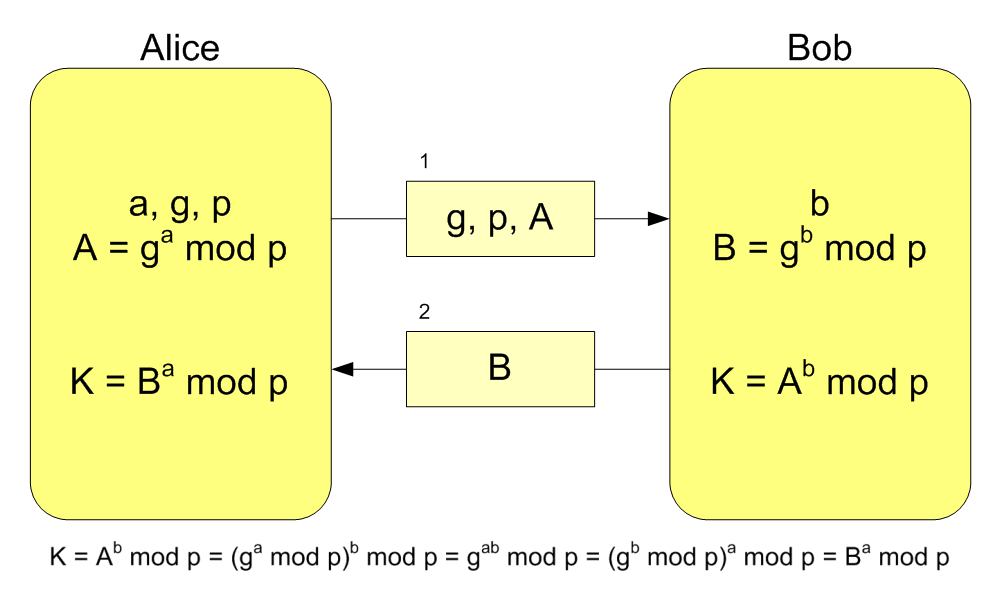
\includegraphics[width=0.6\textwidth]{2dh-hw4-1699981.png} % adjust width
	\caption{\textit{Diffie -- Hellman key exchange (from Wikimedia Commons)}} % optional
	\label{fig:2dh}
\end{figure}

Alice and Bob now share the common and secret key \textit{K}. What happens if also Carol (C) wants to join the process?

\section{DH - Three parties}
Now also Carol wants to share the secret key \textit{K}. She decides a secret value \textit{c}, as Alice and Bob did in the first case.

\begin{enumerate}
	\item Alice picks a prime number \textit{p} and decides the group \textit{g}, sending them to Bob and Carol.
	\item Alice computes $g^a$ and sends it to Bob.
	\item Bob can now compute $g^{ab}$ and sends it to Carol.
	\item Carol computes $g^{abc}$ and is the first one of the group to have the final secret key \textit{K}
\end{enumerate}
What about Bob and Alice? They do not have enough informations to derive the key. Carol, instead, who has the final key, cannot send it back to Bob and Alice, since the channel is insecure. A simple workaround is this:

\begin{enumerate}
	\item Bob computes $g^b$ and sends it to Carol, who forwards to Alice $g^{bc}$
	\item Alice can now compute $g^{bca}$ = \textit{K}
	\item In order to provide also to Bob the key, Carol sends to Alice $g^c$, who forwards to Bob $g^{ca}$
	\item Finally Bob computes $g^{cab}$ = \textit{K} and the process can terminate.	
\end{enumerate}
So the idea here to handle the 3 parties protocol is to share partial computations among parties. This process can be generalized for n parties, with n greater than 3.

\subsection{Security and MITM}
The original DH method does not provide any form of authentication: this results in a critical vulnerability and exposes the parties to Man in the middle (\textbf{MITM}) attacks. In particular, if Alice and Bob want to agree a common key K, the attacker Trudy can agree a key K1 with Alice and a key K2 with Bob, pretending to be Alice when communicating with Bob and vice-versa with Alice. Every single message from Alice to Bob can be decrypted by Trudy, who then can forward whatever she wants to Bob. This security issue can be easily overcome if we use variants of DH that provide authentication.
\newline\newline
\textbf{Note:} In the next sections I will always consider the authenticated DH, i.e. DH + a secure authentication method.

\subsubsection{MITM on a single link}
Say the attacker can sniff packets over the link from Alice to Bob. He is then able to see $g^a$ and $g^{ac}$. We should also assume that the attacker can forge packets; however, he cannot derive in any way the third exponent \textit{b}, that is the secret number picked by Bob; this kind of attack is unsuccessful as long as \textit{b} is not compromised.
\subsubsection{MITM on a single user}
What happens if the attacker can sniff all packets from and to Alice? He is able to collect $g^a$, $g^{bc}$, $g^{ac}$. Again, the attacker still lacks some crucial informations to derive the secret key \textit{K}: in this case the protocol is secure if both \textit{a} and \textit{b} remain secret (not only \textit{b} as in the previous case).  

\subsection{Performance}
\label{sec:3-performance}
DH is known to provide a very efficient way to share a key between two parties, since both Alice and Bob have to compute 2 exponentiations and exchange only 2 messages. With 3 parties the process is not that simple: in fact, we have that each party has to compute 3 exponentiations for a total of $3^2 = 9$ exponentiations (quadratic, as it will be pointed out later). Moreover, also the number of exchanged messages increases, since for each computation the partial value is forwarded to at least another party.

\subsection{A spurious alternative}
A simple alternative, despite a bit \textit{spurious}, could be using DH to let Alice and Bob agree on a key \textit{K1} and also Alice and Carol on the key \textit{K2}. Now Alice generates autonomously a key \textit{K} and sends it to Bob encrypted with \textit{K1} and so does for Carol, encrypting it with \textit{K2}. This is not a pure DH approach, since the final shared key has been decided only by Alice: it requires 8 exponentiations (4 by Alice, 2 by Bob, 2 by Carol) instead of 9. The number of exchanged messages in this case is 2 (Alice and Bob) + 2 (Alice and Carol) + 1 (Alice to Bob) + 1 (Alice to Carol) = 6

\section{DH - N parties}
In this section we see how the DH method can be generalized to allow n parties to share a common key K. As seen before, every user \textit{i} has to choose a secret number (exponent) $e_i$; the secret key K is equal to $ g^m$, where $m:= \prod_{i=1}^{n} e_i$. Since partial computations can be sent over the insecure channel, because even with them the attacker cannot derive m (nor K of course), a simple strategy to reach the goal is this:

\begin{enumerate}
	\item Arrange the users in a circle. Now every user \textit{i} sends to his "next" (i+1 mod N) the partial $g^{e_i}$.
	\item At this point everyone forwards the key received from his "previous", after exponentiating it to $e_i$.
	\item The process terminates after N rounds.
\end{enumerate}
The idea here \cite{Wikipedia} is that each user can add his contribute to partial keys, applying a transformation (exponentiation to $e_i$) that cannot be performed by anyone else.

\begin{figure}[!ht]
	\centering % optional
	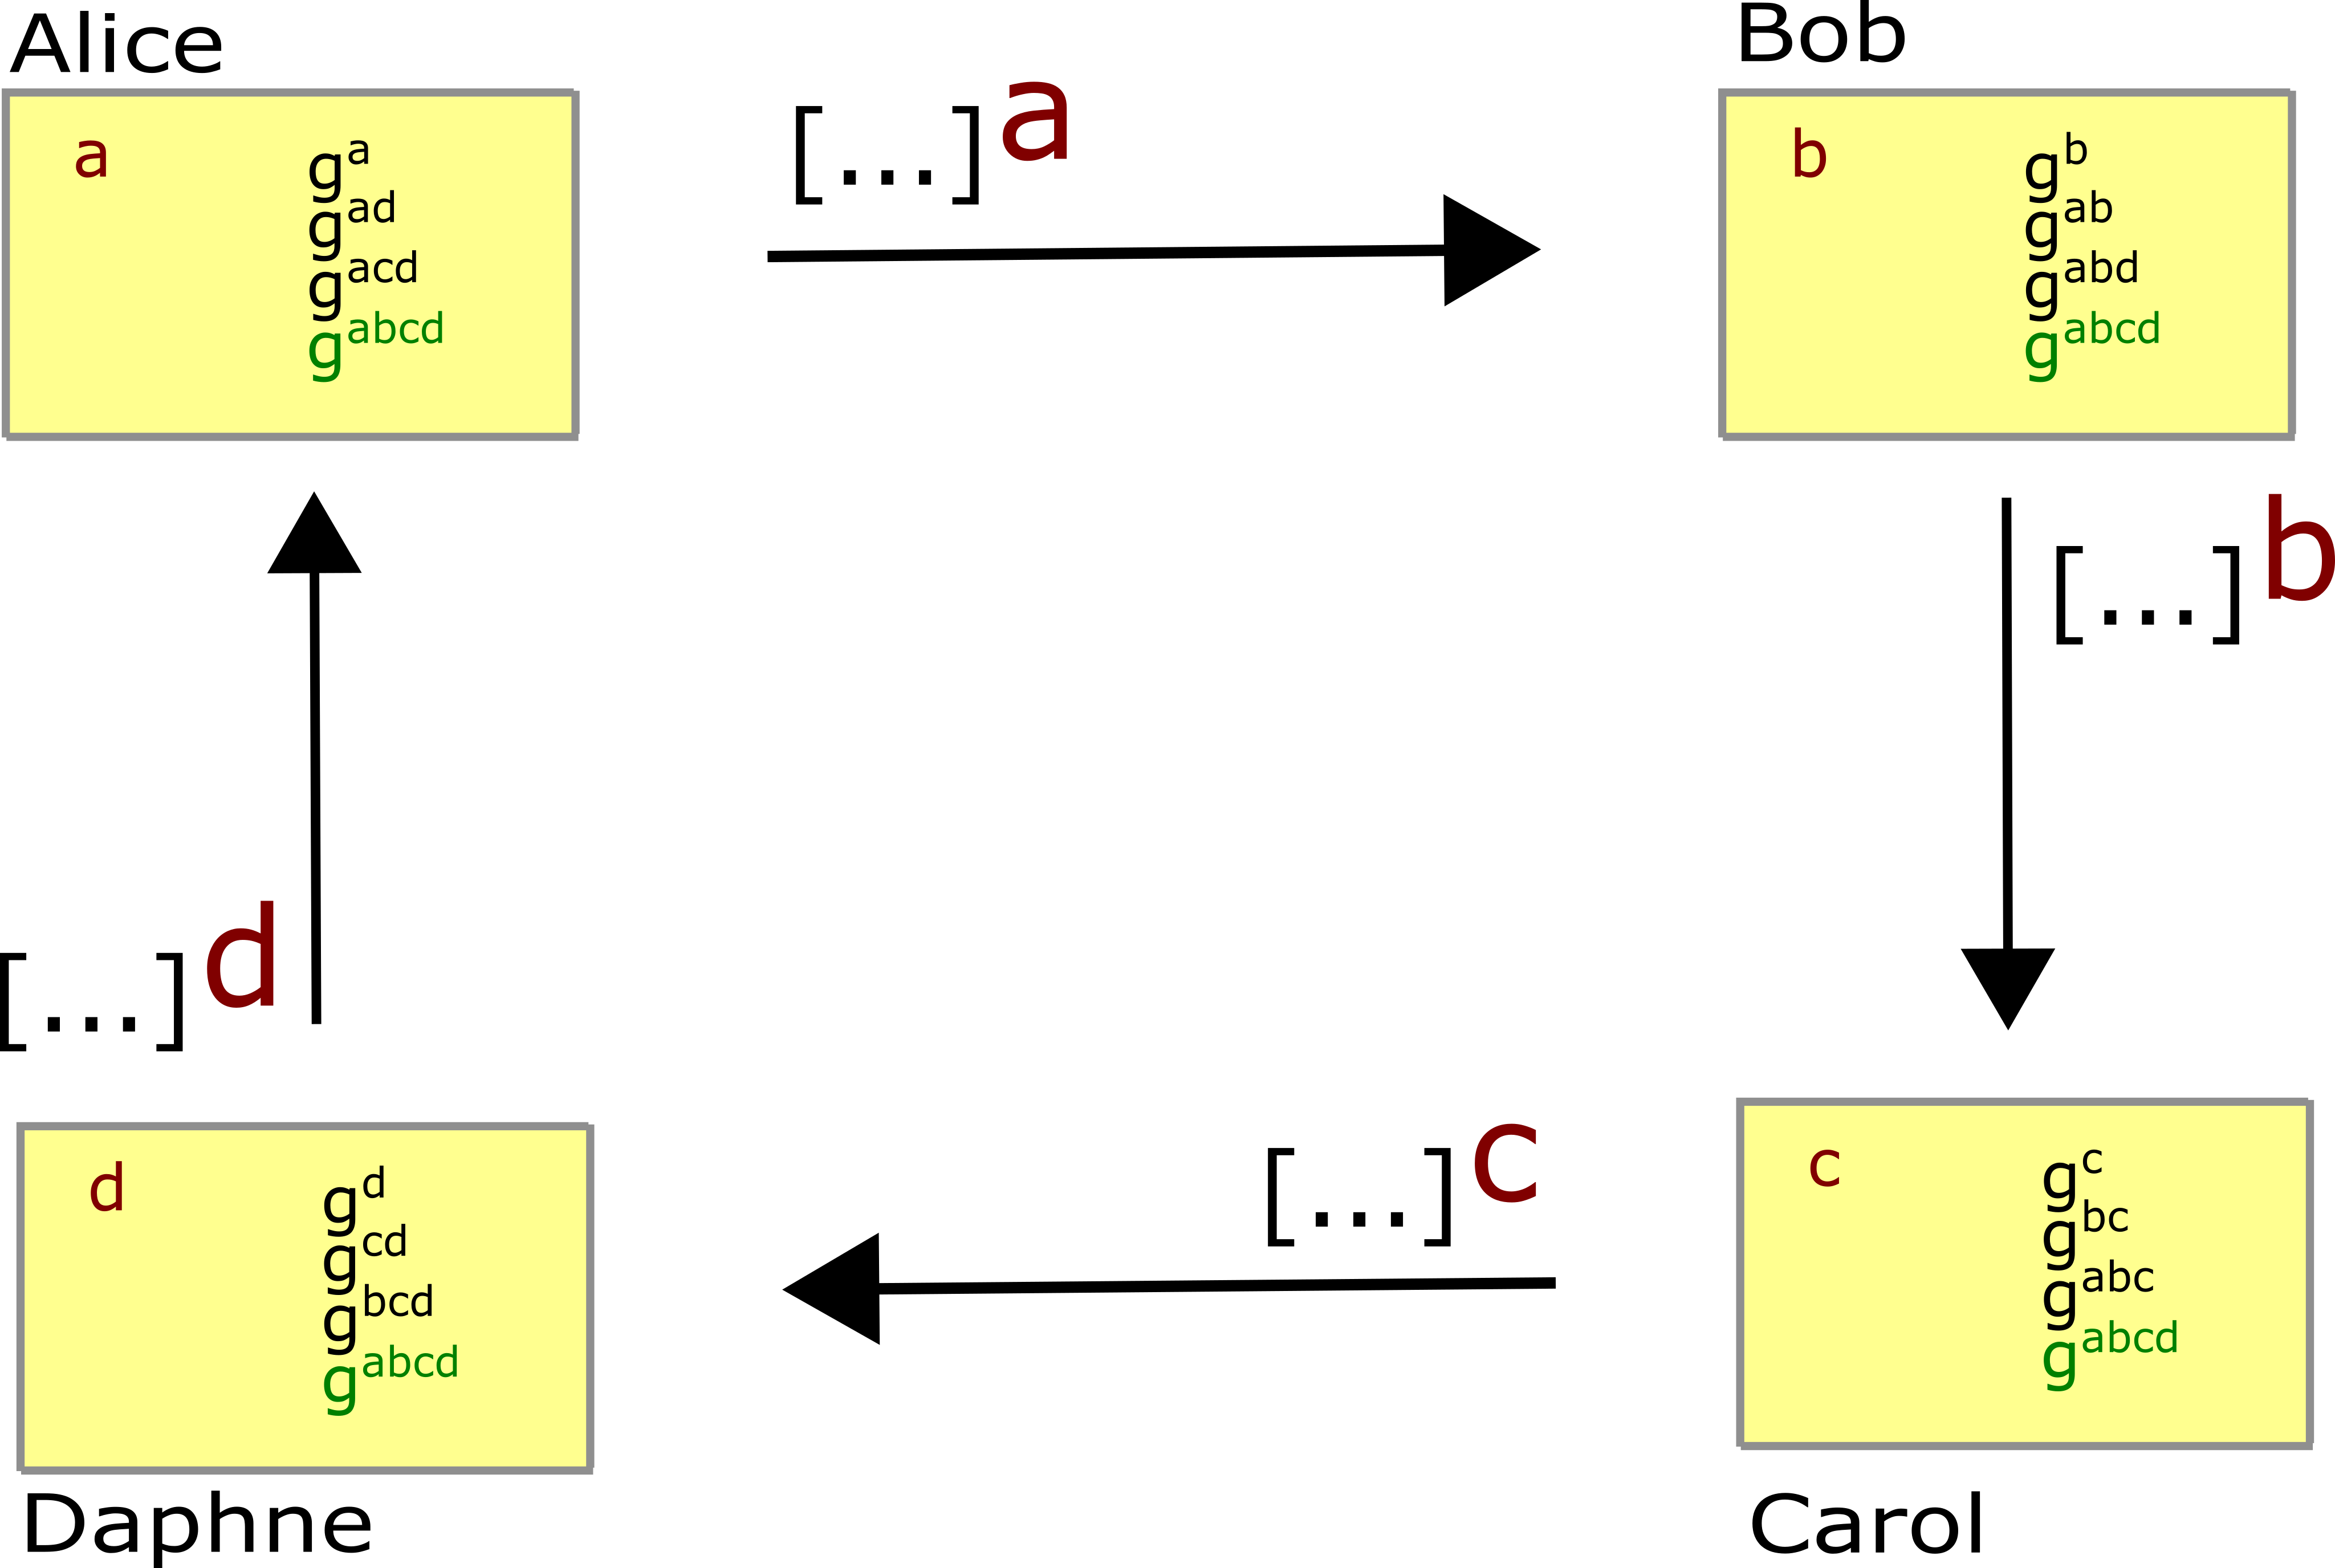
\includegraphics[width=0.7\textwidth]{4dh-hw4-1699981.png} % adjust width
	\caption{\textit{Diffie -- Hellman key exchange for 4 parties}} % optional
	\label{fig:4dh}
\end{figure}

\subsection{Security and MITM}
Again we focus on the authenticated DH schema.

\subsubsection{MITM on a single link}
The attacker can only sniff packets from party \textit{$user_i$} to \textit{$user_{i+1}$}. But the final key is never shared between two adjacent users, and all the partial computations shared through the channel, despite quite numerous, are not enough to derive the key. If the exponent $e_{i+1}$ is compromised, however, the attacker can derive the key since in the final round \textit{$user_i$} sends to \textit{$user_{i+1}$} a partial key $\widetilde{K}$ that exponentiated to $e_{i+1}$ produces K. 

\subsubsection{MITM on a single user}
Again this attack is unsuccessful as long as $e_i$ and $e_{i+1}$ remain secret. This is due to the fact that the attacker can sniff both $\widetilde{K_i}$ and $\widetilde{K_{i+1}}$, where $K = \widetilde{K_i} ^ {e_i}$ 

\subsection{Performance}
Each user performs N exponentiations, so the total number of exponentiations is quadratic (cfr. section \ref{sec:3-performance}). It is possible, however, to reduce the number of exponentiations with a \textit{Divide and Conquer} approach \cite{Wikipedia}, thus resulting in a logarithmic number of operations per user.


\begin{thebibliography}{10}
		
	\bibitem{Wikipedia}
	\textsl{Wikipedia Cryptography Portal} \\
	\textit{https://en.wikipedia.org/wiki/Portal:Cryptography}
	
\end{thebibliography}

\end{document}
